
\section{Introduction}
\subsection{Overview}
% Vehicle volume in the Philippines has worsened uncontrollably. In 2023, there were 1.4 million vehicles currently registered in the Philippines, an increase of 7.63\% over the previous year. MMDA has been proposing a lot of policies over the years; their recent implementation is their EDSA Carousel program, where busses will have their own dedicated lane, and separated from rest of the lanes with barriers. Overall, this has improved commute times from bus riders and encouraging a lot of non-commuters to use these as well. While the general objective of this program has been achieved, the experience to ride one is one of the challenges the riders are facing. The fact that to enter into the carousel, you'll have to cross the road into the middle lane and be exposed to the elements while waiting. And the fact that private vehicles are able to enter into the bus lanes makes everything more complicated. MMDA has been proposing piecemeal solutions to ease our traffic woes, but none of them have been done with extended studies and simulation of the policies. Several simulations prove that using a dynamic approach to solving traffic issues deliver better experience and commute experience than static rulesets.

The rapid increase in vehicle volume in the Philippines has exacerbated traffic congestion to unprecedented levels. In 2023, the country recorded 1.4 million registered vehicles, reflecting a significant 7.63\% increase from the previous year. Over the years, the Metropolitan Manila Development Authority (MMDA) has implemented various traffic management policies to address these challenges. One of their most notable initiatives is the EDSA Carousel program, which allocates dedicated bus lanes separated from other lanes by barriers. This initiative has successfully reduced commute times for bus riders and encouraged more commuters to shift to public transportation.

However, despite its benefits, the program faces significant challenges. Accessing the carousel requires commuters to cross multiple lanes to reach the central bus stops, leaving them exposed to environmental elements and safety hazards. Additionally, unauthorized entry of private vehicles into the bus lanes further complicates traffic dynamics. While the MMDA continues to propose incremental solutions to alleviate congestion, these efforts often lack comprehensive studies and simulations to evaluate their long-term effectiveness.

Research shows that dynamic approaches to traffic management, supported by advanced simulations, can deliver superior results compared to static rule-based systems. This paper explores the potential of such methods in creating more efficient and effective traffic policies tailored to the unique challenges of the Philippines.

% \subsection{Objectives}
% \subsection{Scope and Limitations}

\section{Related Works}
To optimize the flow of traffic in intersections, traffic light systems must be able to optimize their scheduling or control signals based on multiple factors. In this section, describes the methodologies applied to dynamically manage traffic light signals, ranging from traditional to machine learning approaches.
% Typically, the body of a paper is organized into a hierarchical
% structure, with numbered or unnumbered headings for sections,
% subsections, sub-subsections, and even smaller sections.  The command
% \texttt{{\char'134}section} that precedes this paragraph is part of
% such a hierarchy.\footnote{This is a footnote.} \LaTeX\ handles the
% numbering and placement of these headings for you, when you use the
% appropriate heading commands around the titles of the headings.  If
% you want a sub-subsection or smaller part to be unnumbered in your
% output, simply append an asterisk to the command name.  Examples of
% both numbered and unnumbered headings will appear throughout the
% balance of this sample document.

% Because the entire article is contained in the \textbf{document}
% environment, you can indicate the start of a new paragraph with a
% blank line in your input file; that is why this sentence forms a
% separate paragraph.

% \subsection{Type Changes and {\itshape Special} Characters}

% We have already seen several typeface changes in this sample.  You can
% indicate italicized words or phrases in your text with the command
% \texttt{{\char'134}textit}; emboldening with the command
% \texttt{{\char'134}textbf} and typewriter-style (for instance, for
% computer code) with \texttt{{\char'134}texttt}.  But remember, you do
% not have to indicate typestyle changes when such changes are part of
% the \textit{structural} elements of your article; for instance, the
% heading of this subsection will be in a sans serif\footnote{Another
%   footnote here.  Let's make this a rather long one to see how it
%   looks.} typeface, but that is handled by the document class file.
% Take care with the use of\footnote{Another footnote.}  the
% curly braces in typeface changes; they mark the beginning and end of
% the text that is to be in the different typeface.

% You can use whatever symbols, accented characters, or non-English
% characters you need anywhere in your document; you can find a complete
% list of what is available in the \textit{\LaTeX\ User's Guide}
% \cite{Lamport:LaTeX}.

\subsection{Traffic Light Control Systems}
A recent study utilized reinforcement learning, particularly deep-policy gradient, and value-function-based reinforcement learning, to train the agent to select the most optimal control action. They were able to prove that their methods work in a traffic network simulated in the simulation of an urban mobility traffic simulator, without suffering from instability issues during the training process \cite{mousavi2017traffic}.

% Wan 2018
Another method via a value-based- deep reinforcement learning model, which is modified from the deep Q-Learning Network (DQN)algorithm, was implemented on adaptive signal control \cite{wan2018value}. The agent was trained in a micro-simulator called VISSIM at an isolated intersection. This method generates an action that leads to an optimal estimated value within a finite set as the agent’s policy. The study shows that the agent outperforms a fixed timing plan in all testing cases by reducing the system's total delay by 20\%.

%Nishi 2018
Graph Convolutional Neural Networks (GCNNs) can be applied to handle and oversee multiple traffic light controls. Nishi et al. conducted research where they utilized GCNNs in a multi-intersection network to automatically extract features and also take into account the traffic characteristics between distant roads by layering multiple neural network layers.\cite{nishi_traffic_2018}

% Tang 2020
A new approach was proposed that used semi-supervised double dueling broad reinforcement learning now in use in smart cities \cite{tang2020semi}. With their method, they significantly reduced waiting time by about 11.7\% of the average waiting time to the comparative approach. The agent is rewarded for reducing its total cumulative waiting time of consecutive time steps.

% Chu 2020
Chu et al. proposed an algorithm called Multi-Agent Advantage Actor-Critic (MA2C), which is a multi-agent variant of the classical independent Advantage Actor-Critic (A2C). This study proposed dividing the overall traffic controls into multiple local RL agents. The significant contribution of this proposal is to create an optimal and robust model for each agent by avoiding the large dimensionality of the environment. \cite{chu_multi-agent_2020}

% Han 2024
Recently, the attention mechanism from transformers was also introduced as a new Reinforcement Learning-based strategy for Large-Scale Adaptive Traffic Signal Controls. This approach integrates the attention mechanism into a multi-agent proximal policy optimization (MAPPO) RL model to enable more effective, scalable, and stable learning in a complex ATSC environment. The results by the author claim that the approach was able to learn stable and sustainable policies to achieve lower congestion and claimed to outperform other state-of-the-art approaches \cite{han_attention_2024}.

\subsection{Traffic Simulators}
Traffic simulators are essential tools for evaluating and optimizing traffic management strategies. Two widely used traffic simulators are Simulation of Urban MObility (SUMO) and Verkehr In Städten - SIMulationsmodell (VISSIM). SUMO is an open-source, highly portable, microscopic, and continuous road traffic simulation package designed to handle large road networks. It allows for the simulation of various traffic scenarios and supports the integration of external control algorithms. VISSIM, on the other hand, is a proprietary microscopic multi-modal traffic flow simulation software. It provides a detailed and realistic representation of traffic operations and is often used for traffic engineering and planning purposes. Both simulators are instrumental in testing and validating traffic control systems, including those based on reinforcement learning and other advanced methodologies.
\subsection{Reinforcement Learning}
\section{Conceptual Framework}
\subsection{Complex Systems}

Complex systems refer to the study of individual elements or agents interacting with each other, often from a microscopic perspective. One of the key concepts studied in complex systems is the collective behavior of these agents, which might not make sense if you observe the individual parts alone. For example, ant colonies exhibit complex behavior despite each drone carrying out seemingly basic actions, such as gathering food, caring for the queen and larvae, and defending the colony from intruders.\cite{newman_complex_2011}

While these actions may suggest that ants lack high-level thinking, a macroscopic view reveals that they organize themselves in complex ways, building individual rooms in their colony, developing communication systems to indicate nearby food, and collectively attacking intruders without high-level communication. This perspective allows us to study these elements differently and observe emerging behaviors when the environment changes.

The concept of complex systems is also heavily used in traffic studies, where even slight policy changes can affect the entire behavior of drivers and pedestrians. Drivers and pedestrians have a single objective – to travel from point A to point B – but they experience different journeys depending on their preferred transport method (e.g., cars, buses, bikes, trains, or walking). Each of these methods is heavily influenced by how the government implements policies. This study aims to observe both the positive and negative emergence of behaviors resulting from different policies.

\subsection{Agent-Based Modelling}
Agent-based modeling (ABM) is a powerful approach for simulating complex systems composed of autonomous, interacting entities called agents. Andy Landsdowne (2006) defined an 'agent' as "\textit{a computer system that is situated in some environment, and that is capable of autonomous action in this environment in order to meet its designed objective}" (p.22) \cite{lansdowne_multi-agent_2006}. Agents sense their surroundings through inputs and take actions based on preconditions and goals to influence their environment, mimicking the behaviors of the entities they represent.

In traffic simulation, agents must be implemented via multi-agent systems (MAS), where each agent interacts with others. When agents are given simple behaviors and simulated as a group, new behaviors often emerge that were not explicitly programmed, known as emergent phenomena \cite{Lindsey2002}. This interaction is crucial for modeling realistic traffic patterns and understanding the dynamics within a transportation system.

ABM allows us to model individual vehicles and other elements of the transportation system as discrete agents, each with their own properties and behaviors. This bottom-up approach enables the emergence of realistic traffic patterns and behaviors from the interactions of these agents, providing valuable insights into traffic dynamics and management strategies.

\subsection{Traffic Dynamics}
Traffic Dynamics is a field of study that focuses on the interactions and behaviors that occur within transportation systems. It involves the movement of vehicles, pedestrians, and other entities within a dynamic urban environment. This framework draws upon principles from various disciplines, including transportation engineering, urban planning, and behavioral psychology, to understand the intricate dynamics that govern traffic patterns, congestion phenomena, and the optimization of mobility networks. By exploring factors such as vehicle movement, traffic control mechanisms, human behavior, and environmental influences, Traffic Dynamics provides a comprehensive way to analyze and improve the efficiency, safety, and sustainability of transportation systems in modern urban landscapes.

Ross (1988) mentioned that for the purposes of control, simulation, and general understanding, a description of traffic in terms of continuous and differentiable quantities is needed and developed a formulation that is more qualitatively "correct." According to the study, there are 3 traffic variables that can form 2 relationships:

\begin{enumerate}
    \item \textit{k} = vehicular density (veh/mi)
    \item \textit{v} = (local space-mean) speed (mph)
    \item \textit{Q} = traffic volume (veh/hr)
\end{enumerate}

The first known relationship is inherent in the definitions of volume, density, and speed as modeled in the equation \eqref{eq:first_rel}
\begin{equation}
    Q = kv
    \label{eq:first_rel}
\end{equation}

The second relationship, the continuity of vehicles, was pointed out by Lighthill and Whitham (1955) as an equation in \eqref{eq:second_rel}.
\begin{equation}
    \frac{\partial k}{\partial t} + \frac{\partial Q}{\partial x} = S(x, t)
    \label{eq:second_rel}
\end{equation}

where $\frac{\partial}{\partial t}$ and $\frac{\partial}{\partial x}$ indicate partial differentiation with respect to time \textit{t} and with respect to the location along the road \textit{x}, respectively, and $S(x, t)=$ vehicles entering (positive) or leaving (negative) the roadway (veh/mi-hr).

As equations \eqref{eq:first_rel} and \eqref{eq:second_rel} do not constitute a complete formulation of traffic flow, Ross determined that a third relationship is needed.

\subsection{Traffic Simulations}
\section{Traffic Simulation}
Drew (1968) describes simulation as a dynamic representation of some part of the real world achieved by building a computer model and moving it through time. Fishburn et al. also described traffic simulation as a valuable decision-making tool for evaluating transport infrastructure and systems.  Concepts like agent-based modeling and path-finding allow us to design an automated behavior for virtual drivers and pedestrians \cite{drew1968traffic}.

Traffic Simulations are especially beneficial in testing the effectiveness of policies. Wirtz (2005) utilized simulation to test traffic incident management strategies without explicitly implementing the policy in the real world. In his study, he was able to identify the bottlenecks of the policies in a national highway in California and provided several recommendations from the insights, such as to increase highway capacities of perpendicular artery roads and retiming and resynchronization of traffic signals also help in decongesting the affected route \cite{wirtz2004using}.

According to Backfrieder's study in 2013, Traffic Simulators are crucial components of intelligent traffic management systems. Their research focuses on a more detailed model for simulating traffic that's closer to reality. They claim that this approach allows for analyzing more granular factors such as fuel consumption, travel time, and travel distance. Moreover, it can examine how these factors can affect driver behavior when congestion information is received earlier and can bypass congested road sections.

\section{Methodology}

\subsection{Data Collection}
We will collect CCTV video data of BGC intersections from sources like Township Analytics or BGC traffic authorities. Identifiable information such as license plates and faces will be anonymized as they are not relevant to the research.

Additionally, high-level traffic data from ArcGIS, Google Maps, or Waze will be gathered to analyze traffic patterns, identify congestion areas, and peak times. Traffic light phase data will also be requested to initialize the SUMO environment.

The CCTV data will be processed using Object Detection Models like YOLO or Faster RCNN to detect vehicle positions. This data will help build an initial ABM model replicating traffic patterns. Vehicles will be tracked by superimposing masks on CCTV frames to mark their origin and destination points as they move through intersections.

\begin{figure}
    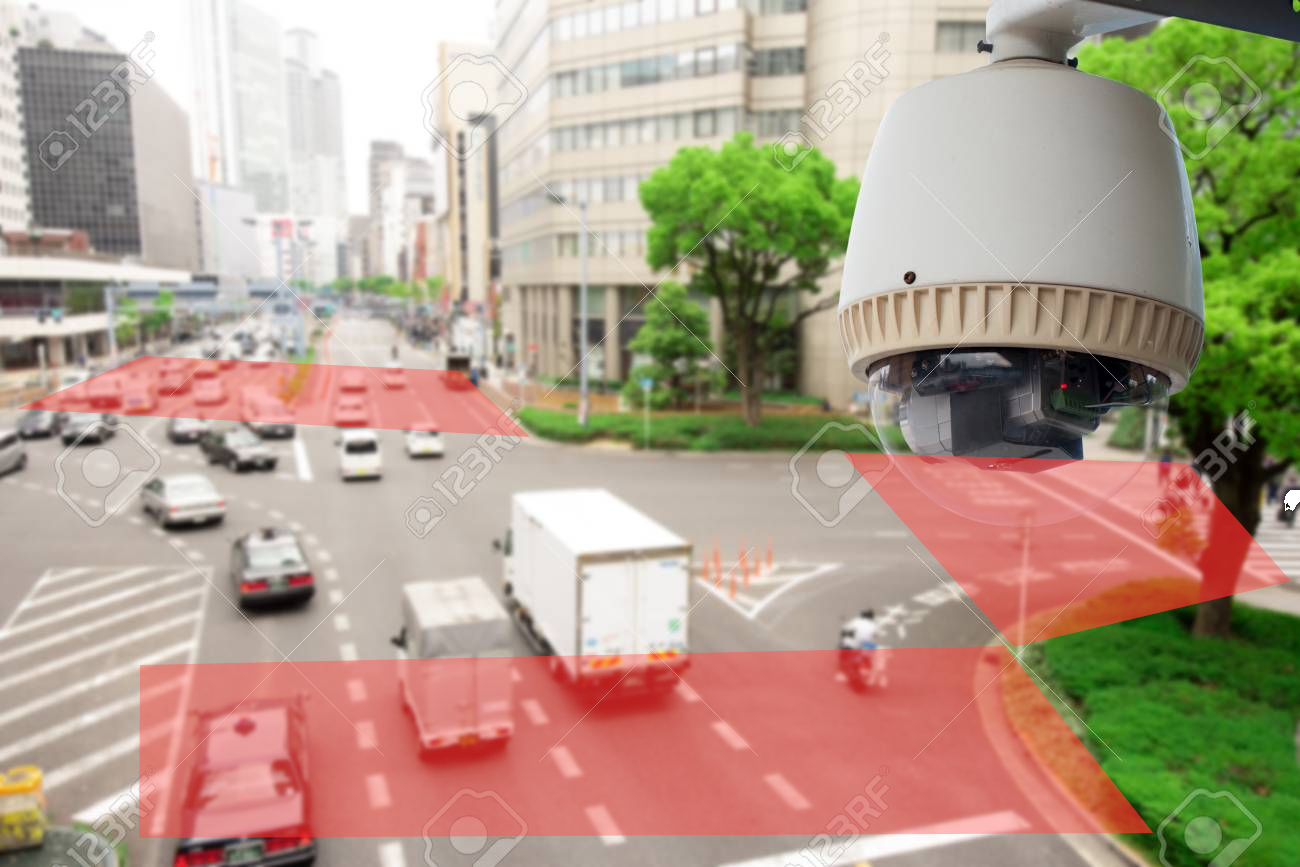
\includegraphics[height=1in, width=1.5in]{figures/cctv_frame_mask.png}
    \caption{A sample black and white graphic that has
    been resized with the \texttt{includegraphics} command.}
\end{figure}

\subsection{Environment Design}
In this study, we utilized the SUMO simulator for our enviroment. The reason we chose this is because it was the most common platform to train and implement agent based modelling via the TraCI API. TraCI API is an interface used to connect the environment to a programming language such as Python.

% Insert image here

We based off our initial environment mirroring the intersection around Uptown Mall in BGC, Philippines. The reason we chose this is the proximity and ease of access from the location of the author. We also believed this is the perfect area to observe different traffic patterns, and driver behaviors to model in the environment as well as the varying transport modes found in this area.

The environment itself consists of 4 legs, each with 3 lanes: 2 regular lanes, and a bike lane, which is very common in BGC. We then implemented sub-lanes to simulate the lane filtering behavior as well as vehicles veering off in different lanes aggressively. This implementation also simulates the lane filtering behaviors commonly found in motorcycles. Traffic light phase design is a rotating mechanism, which means that for every phase only 1 leg at a time allows vehicles to go through. Right turns are always available for all vehicles as per the design of the junctions in BGC. 

\subsection{Modelling Agents}

The agent behaviors were initially derived from the default models provided by the SUMO simulator. These models served as a foundation for the customization process. We tailored the attributes of each vehicle type by modifying key parameters such as dimensions and lane-changing behaviors. This customization ensures that the simulated traffic environment closely mirrors real-world conditions.

In the next phase, the agents' behaviors will be enhanced further through the integration of Hidden Markov Models (HMMs). This approach allows us to predict future behaviors based on the agents’ current states. The probability of state transitions within the HMM framework will be informed by data collected from closed-circuit television (CCTV) systems. By analyzing this CCTV data, we aim to capture realistic behavioral patterns and use them to refine the simulation.

Currently, we have modeled three distinct types of transport vehicles: cars, motorcycles, and bicycles. Each category has been meticulously designed to account for its unique characteristics and interactions within the traffic system. Additionally, we incorporated pedestrian dynamics into the simulation, primarily using the default JuPedSim model available in SUMO. This inclusion enables us to evaluate the impact of pedestrian movement on traffic patterns and overall flow.

Pedestrian crossings have been implemented at all four legs of the simulated intersection. For an added layer of realism, the pedestrian crossing adjacent to a vehicle lane turns green simultaneously with the green signal for that specific vehicle lane. This design aims to emulate real-world traffic scenarios where pedestrian and vehicular flows are synchronized, further enhancing the validity of the simulation.

\subsection{Traffic Light Management Agent}

To train our Traffic Management agent, we employed Reinforcement Learning (RL) techniques to determine the most optimal traffic light policy for various conditions. For our initial proof of concept (POC), we utilized stable baselines RL frameworks to establish a foundational approach. The TraCI API was employed to seamlessly extract data from the SUMO simulator, and build those as observation spaces for our RL models.

\subsubsection{Observation Spaces}

For the observation spaces, we implemented the following features to provide the agent with a comprehensive understanding of the traffic conditions:

\begin{enumerate}
    \item \textbf{Current Phase Lane}: Represented as a one-hot encoded vector, this feature indicates the current active phase of the traffic light, allowing the agent to understand which lanes are currently allowed to move.
    \item \textbf{Minimum Green Duration}: A binary indicator that shows whether the current phase duration has met the minimum green time requirement. This helps the agent ensure that each lane receives a fair amount of green light time.
    \item \textbf{Lane Density}: This feature measures the density of each lane by calculating the ratio of the number of incoming vehicles to the total capacity of the lane. It provides the agent with information about how congested each lane is.
    \item \textbf{Lane Queue Length}: Indicates the number of vehicles in each lane that are moving at speeds below 0.1 miles per hour, effectively capturing the length of the queue and helping the agent identify lanes with significant traffic buildup.
\end{enumerate}


\subsubsection{Action Spaces}
For the action spaces, the agent is free to pick how long the next phase would be.

\subsubsection{Reward Functions}
For the reward functions, the following are implemented:
\begin{enumerate}
    \item \textbf{Diff Waiting Time} - Produces a reward if the waiting time is improved from the last measure.
    \item \textbf{Average Speed} - Produces a reward that increases as the average speed of the network improves.
    \item \textbf{Queue Time} - Produces a reward when the number of incoming vehicles is less than the capacity of each lane.
    \item \textbf{Lane Pressure} - Produces a reward by computing the difference between the outgoing and incoming vehicles in each lane.
    \item \textbf{Pedestrian Waiting Time} - Produces a reward by checking if the pedestrian waiting time has improved from the last measure.
\end{enumerate}

\section{Preliminary Results}
While the project is still in progress, we are already observing the potential benefits of using reinforcement learning for traffic management, even though the current simulation environment does not yet fully capture real-life traffic patterns. 

We initially collected the historical system mean waiting time as a metric, and we observed that the mean was becoming more stable as the agent learned to optimize the traffic light phases. This stabilization indicates that the agent is effectively learning to manage traffic flow and reduce congestion.

As we continue to collect more accurate data, we are simultaneously developing and refining our reinforcement learning agent. This parallel approach allows us to establish a robust workflow, ensuring that as new data is collected and ingested, we can continuously improve the model and enhance its effectiveness in managing traffic dynamics.

% Put graphs here.

\section{Future Works}

Although the study is still ongoing, we aim to expand its scope to cover a significantly larger area, ideally encompassing the entirety of Bonifacio Global City (BGC). This expansion would necessitate the collection of an even greater volume of data, as we anticipate varying traffic behaviors across different intersections within BGC. Capturing these variations is crucial to developing robust models that can address the unique characteristics of each junction effectively.

Moreover, as we scale up, we plan to transition to a multi-agent reinforcement learning (MARL) methodology. This shift is in line with standard practices for managing multiple interconnected traffic signals, as MARL allows for the efficient coordination of individual traffic lights within a broader network. By leveraging MARL, we can model interactions between agents and address the complexities of multi-intersection traffic management more effectively.

However, implementing MARL comes with significant computational demands. Training multiple agents simultaneously within a reasonable time frame requires high-performance hardware. As such, we anticipate the need for multi-GPU and multi-CPU systems, which will require additional investment to ensure the success of this next phase of the study.
\appendix
%Appendix A
% \section{Headings in Appendices}
% The rules about hierarchical headings discussed above for
% the body of the article are different in the appendices.
% In the \textbf{appendix} environment, the command
% \textbf{section} is used to
% indicate the start of each Appendix, with alphabetic order
% designation (i.e., the first is A, the second B, etc.) and
% a title (if you include one).  So, if you need
% hierarchical structure
% \textit{within} an Appendix, start with \textbf{subsection} as the
% highest level. Here is an outline of the body of this
% document in Appendix-appropriate form:
% \subsection{Introduction}
% \subsection{The Body of the Paper}
% \subsubsection{Type Changes and  Special Characters}
% \subsubsection{Math Equations}
% \paragraph{Inline (In-text) Equations}
% \paragraph{Display Equations}
% \subsubsection{Citations}
% \subsubsection{Tables}
% \subsubsection{Figures}
% \subsubsection{Theorem-like Constructs}
% \subsubsection*{A Caveat for the \TeX\ Expert}
% \subsection{Conclusions}
% \subsection{References}
% Generated by bibtex from your \texttt{.bib} file.  Run latex,
% then bibtex, then latex twice (to resolve references)
% to create the \texttt{.bbl} file.  Insert that \texttt{.bbl}
% file into the \texttt{.tex} source file and comment out
% the command \texttt{{\char'134}thebibliography}.
% % This next section command marks the start of
% % Appendix B, and does not continue the present hierarchy
% \section{More Help for the Hardy}

% Of course, reading the source code is always useful.  The file
% \path{acmart.pdf} contains both the user guide and the commented
% code.

% \begin{acks}
%   The authors would like to thank Dr. Yuhua Li for providing the
%   MATLAB code of the \textit{BEPS} method.

%   The authors would also like to thank the anonymous referees for
%   their valuable comments and helpful suggestions. The work is
%   supported by the \grantsponsor{GS501100001809}{National Natural
%     Science Foundation of
%     China}{http://dx.doi.org/10.13039/501100001809} under Grant
%   No.:~\grantnum{GS501100001809}{61273304}
%   and~\grantnum[http://www.nnsf.cn/youngscientists]{GS501100001809}{Young
%     Scientists' Support Program}.

% \end{acks}
